\documentclass[11pt]{article}

\usepackage[T1]{fontenc}
\usepackage{lmodern}
\usepackage{amsmath}
\usepackage{amssymb}
\usepackage{mathtools}
\usepackage{microtype}
\usepackage{graphicx}
\usepackage{booktabs}
\usepackage{array}
\usepackage{tabularx}
\usepackage{multirow}
\usepackage{enumitem}
\usepackage{xcolor}
\usepackage{fancyhdr}
\usepackage[margin=1in]{geometry}
\usepackage{hyperref}
\hypersetup{
  colorlinks=true,
  linkcolor=blue!70!black,
  citecolor=green!50!black,
  urlcolor=blue!80!black,
  bookmarksnumbered=true,
  pdfauthor={Ioannis Tsiokos},
  pdftitle={To Wake a Stone with Six Birds: A Life is A Theory}
}
\usepackage{cleveref}
% Consistent lowercase references
\crefname{section}{section}{sections}
\crefname{table}{table}{tables}
\crefname{figure}{figure}{figures}
\usepackage{natbib}
\usepackage{tikz}
\usetikzlibrary{arrows.meta, positioning}


% Prevent widows and orphans
\widowpenalty=10000
\clubpenalty=10000
\raggedbottom

% Macro block (minimal; extend later)
\newcommand{\Tpkg}{\mathcal T}
\newcommand{\Audit}{\mathcal A}
\newcommand{\KL}{D_{\mathrm{KL}}}
\newcommand{\TV}{\mathrm{TV}}
\newcommand{\Sig}{\Sigma}
\newcommand{\SAFE}{\textsc{safe}}
\newcommand{\SUGG}{\textsc{suggestive}}
\newcommand{\NEG}{\textsc{negative}}

\title{To Wake a Stone with Six Birds: A Life is A Theory}
\author{Ioannis Tsiokos\textsuperscript{1}}
\date{27 January 2026}

\newcommand{\printaffiliation}{%
  \begin{center}
    \small \textsuperscript{1}Automorph Inc., 1207 Delaware Ave \#4131, Wilmington, DE 19806, USA
  \end{center}
}

\fancypagestyle{firstpage}{%
  \fancyhf{}
  \fancyfoot[C]{\scriptsize DOI: \href{https://doi.org/10.5281/zenodo.18394536}{10.5281/zenodo.18394536} \quad \textcopyright\ 2026 Automorph Inc.\ \quad Licensed under CC-BY 4.0 International.}
  \renewcommand{\headrulewidth}{0pt}
  \renewcommand{\footrulewidth}{0pt}
}

\begin{document}
\maketitle
\printaffiliation
\thispagestyle{firstpage}

\begin{abstract}
Empirical work on life-like organization often conflates protocol artifacts with genuine directionality and lacks a disciplined way to state and check claims across descriptive levels. We report a life-focused instantiation of the emergence calculus developed in \citet{tsiokos2026sixbirds} by specifying finite theory packages $\Tpkg=(Z,f,\Sig_f,E,\Audit)$ for two substrates (a particle-based substrate and a neural/meta-layer substrate) and indexing each reported claim to external experimental artifacts via a machine-readable ledger. Across both substrates we (i) calibrate strict null regimes (P3=OFF, P6=OFF) where audit proxies are statistically consistent with zero, reducing false-positive arrow-of-time signals; (ii) demonstrate a separable drive channel (P6) that yields clean null--drive separation in audit proxies under matched controls; and (iii) show that protocol holonomy (P3) changes stroboscopic currents under matched control while remaining a diagnostic rather than a directionality certificate. We further report maintenance/viability proxies---repair performance, traversal requirements, and deadline selection with explicit audit cost---and, in the neural substrate, refined-lens predicate families: stable motif inventories, proto-syntax shifts, and intervention-based dictionary/decoding statistics validated by shift-null significance tests. While the framework allows arbitrarily many theory extensions in the definability sense (adding new lens predicates), we do not claim autonomous open-ended evolution in the ALife sense (indefinite novelty generation under a fixed regime without external steering). Limitations are explicit: audits are proxies (not full path-space KL), idempotence defects are not measured, and formal definability separations are not proved.
\end{abstract}

\vspace{1ex}
\noindent\textbf{keywords:} emergence calculus; directionality; audit proxies; life-like organization; finite theory package; protocol holonomy; nonequilibrium dynamics

\section{Introduction}\label{sec:intro}
A prior framework paper \citep{tsiokos2026sixbirds} proposes an emergence calculus in which empirical claims are organized by a finite theory package $\Tpkg=(Z,f,\Sig_f,E,\Audit)$ and three certificates: stability/objecthood, novelty/extension, and directionality/audit. That framework is intentionally math-only and explicitly defers instantiations. The present work delivers the life-focused instantiation by fixing concrete $\Tpkg=(Z,f,\Sig_f,E,\Audit)$ packages for two substrates and reporting certificate evidence with conservative controls.

\paragraph{Intellectual context and credit.}
While the emergence calculus and contracts used here are our own, this life-focused instantiation was strongly inspired by two adjacent lines of work that emphasize graded, multi-scale agency and the centrality of \emph{interpretation across layers}.
In the diverse-intelligence program, Michael Levin and collaborators argue that the genotype--phenotype relationship is best understood as an active, multi-scale problem-solving and error-correcting process (not merely a static decoder), and they develop substrate-independent characterizations of cognition in terms of remapping and navigating embedding spaces under iterative error minimization \citep{hartl2025evolutionmake,hartl2026remapping}.
In a complementary direction, Bennett's thesis develops a ``stack'' view in which policies at successive abstraction layers carve out stable causal identities and operationally goal-directed behavior (goal-directed in a control-theoretic sense, not ascribed intention) \citep{bennett2025consciousmachines}.
We include this paragraph explicitly because significant parts of our motivation came from these perspectives, even though the present paper does not derive its formalism from them.

\paragraph{Empirical workflow.}
Our empirical workflow is deliberately audit-first: we calibrate strict null regimes in which protocol (P3) and drive (P6) are disabled, and require directionality-relevant audit proxies to be consistent with zero before interpreting any driven behavior as an arrow-of-time signal. We then (i) demonstrate drive separability via P6 under matched null controls, (ii) quantify protocol holonomy effects via matched-control stroboscopic diagnostics without attributing directionality to P3 alone, and (iii) report maintenance and higher-level descriptive structure only where supported by explicit gates, contracts, and shift-null tests.

\paragraph{What ``life-like'' means here.}
Throughout, we use ``life-like'' as shorthand for a limited family of \emph{operational competencies} that can be stated and checked within the emergence-calculus vocabulary: (i) an audited directionality channel that separates cleanly from null controls, (ii) maintenance/repair and perturbation recovery under externally imposed hazards or deadlines with explicit costs, and (iii) at refined lenses, stable predicate families that support controlled readout under explicit gates and shift-null tests. We are not proposing a general definition of biological life, and we do not model reproduction, heredity, or population-level evolution; replication enters only as contextual comparison in the Discussion.

\paragraph{Title intuition.}
Here, ``to wake a stone'' refers to moving from a strictly calibrated null (no protocol, no drive) to a regime with auditable directionality and maintenance under explicit costs; the ``six birds'' name the primitive operations we toggle to make that transition testable rather than rhetorical.

\paragraph{Claim ledger.}
To keep the narrative checkable, every claim used in the paper is indexed in \texttt{assets/claims.yml}, which maps from claim IDs to the precise external tables/contracts in the particle and neural experiment repositories. This paper therefore serves as a worked example of how the emergence-calculus vocabulary can be used to state, audit, and bound life-like claims in complex substrates.

\paragraph{Related work.}
Related efforts toward general theories of life also emphasize constraint-driven universality across scales; for example, Sol{\'e} et al.\ survey six recurring biological constraint families spanning thermodynamics, molecular information, cellularity, development, cognition, and ecosystem organization \citep{SoleEtAl2024Constraints}. In the Discussion we note a suggestive (but non-canonical) one-to-one correspondence between these six families and the six ``birds'' (P1--P6) of the emergence calculus.

\paragraph{Code availability.}
Experiment repositories are available at:
\begin{itemize}[noitemsep,topsep=2pt]
\item Neural substrate: \url{https://github.com/ioannist/six-birds-neural}
\item Particle substrate: \url{https://github.com/ioannist/six-birds-particle}
\end{itemize}

\section{Framework recap (canonical)}\label{sec:framework}
This paper instantiates the emergence calculus developed in the framework paper \citep{tsiokos2026sixbirds}. The framework isolates a \emph{finite theory package} and three logically distinct certificates---stability/objecthood, novelty/extension, and directionality/audit---so that empirical instantiations can be stated and checked without conflating these roles.

\subsection{Finite theory package}\label{sec:framework:tpkg}
A \emph{finite theory package} is a tuple
\[
\Tpkg=(Z, f, \Sig_f, E, \Audit).
\]
Here $Z$ is the microstate space. A \emph{lens} $f:Z\to X$ specifies what is observable at a given descriptive level; it induces a definability structure $\Sig_f$ (equivalently, the partition of $Z$ into the fibers $f^{-1}(x)$). A \emph{completion/packaging endomap} $E:\mathcal V\to\mathcal V$ acts on a chosen description space $\mathcal V$ (for example, distributions over $Z$), and its fixed points $\mathrm{Fix}(E)=\{v\in\mathcal V:\,E(v)=v\}$ are the ``objects'' recognized at that level. Finally, an \emph{audit functional} $\Audit$ provides a nonnegative certificate intended to be monotone under further coarse observation (so coarse-graining should not create false positives) \citep{CoverThomas2006}.
See \cref{fig:tpkg_pipeline} for a schematic.

\begin{figure}[t]
\centering
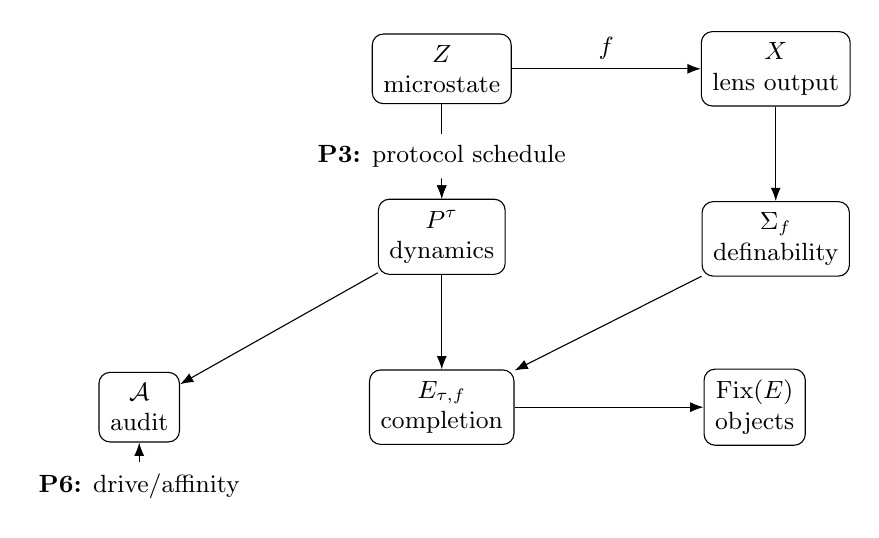
\begin{tikzpicture}[node distance=1.35cm, >=Latex, font=\small]
\tikzstyle{bx}=[draw, rounded corners, inner sep=4pt, align=center]

\node[bx] (Z) {$Z$\\microstate};
\node[bx, right=2.4cm of Z] (X) {$X$\\lens output};
\draw[->] (Z) -- node[above] {$f$} (X);

\node[bx, below=1.2cm of X] (Sig) {$\Sig_f$\\definability};
\draw[->] (X) -- (Sig);

\node[bx, below=1.2cm of Z] (P) {$P^\tau$\\dynamics};
\draw[->] (Z) -- (P);

\node[bx, below=1.2cm of P] (E) {$E_{\tau,f}$\\completion};
\draw[->] (P) -- (E);
\draw[->] (Sig) -- (E);

\node[bx, right=2.4cm of E] (Fix) {$\mathrm{Fix}(E)$\\objects};
\draw[->] (E) -- (Fix);

\node[bx, left=2.4cm of E] (A) {$\Audit$\\audit};
\draw[->] (P) -- (A);

\node[bx, above=0.25cm of P, fill=white, draw=none] (P3lab) {\textbf{P3:} protocol schedule};
\draw[->, dashed] (P3lab) -- (P);

\node[bx, below=0.25cm of A, fill=white, draw=none] (P6lab) {\textbf{P6:} drive/affinity};
\draw[->, dashed] (P6lab) -- (A);
\end{tikzpicture}
\caption{Schematic of the finite theory package $\Tpkg=(Z,f,\Sig_f,E,\Audit)$ and where P3/P6 enter. P3 is treated as a holonomy/protocol \emph{diagnostic} that modifies coarse behavior via protocolized dynamics, while sustained directionality is attributed only when an audit channel separates cleanly (e.g., P6 in \cref{tab:p6_separability}).}
\label{fig:tpkg_pipeline}
\end{figure}

\subsection{Three certificates}\label{sec:framework:certificates}
The framework separates three questions that are often entangled:
\begin{enumerate}[leftmargin=*]
\item \textbf{Stability / objecthood.} A descriptive level exhibits objecthood when its completion rule behaves (approximately) as a closure: applying $E$ does not keep changing the description, and there exist multiple robust fixed points (not a trivial constant map). Empirically, this is typically evaluated through stability/retention proxies rather than claimed by definition.
\item \textbf{Novelty / extension.} Iterating a fixed completion saturates. Strict novelty corresponds to a \emph{theory extension}: changing what is definable (e.g., by adjoining predicates not definable from the prior lens) or changing the completion rule itself. In this paper we use ``novelty'' only in this definability-based sense, not as a synonym for ``interesting dynamics.''
\item \textbf{Directionality / audit.} Directionality is certified by an audit. A canonical example is the path-space arrow-of-time at horizon $T$ \citep{LebowitzSpohn1999,Seifert2012},
\[
\Sig_T(\rho)\;:=\;\KL\!\left(\mathbb P_{\rho,T}\,\middle\|\,\mathcal R_{*}\mathbb P_{\rho,T}\right),
\]
where $\mathcal R$ reverses trajectories. Because $\Sig_T(\rho)$ is a KL divergence it is nonnegative, whereas the finite-window proxy estimators we report can be signed (and occasionally slightly negative) due to accepted-move-only logging, ignored proposal terms, and sampling noise; we interpret them via null calibration, confidence intervals, and clean regime separation rather than as absolute thermodynamic quantities.
In our instantiations we report concrete audits and audit \emph{proxies}, and we are explicit about when a reported quantity is a proxy rather than an exact path-space KL audit.
\end{enumerate}

\subsection{Protocols and the P3 boundary}\label{sec:framework:p3boundary}
Protocol holonomy (primitive P3) is a \emph{diagnostic} describing how coarse behavior can depend on the route by which a closure or update is realized. Protocols can strongly affect coarse currents and stroboscopic statistics, but \textbf{P3 is not itself a directionality certificate}. Under autonomy, if the protocol phase is treated as part of the state (a lifted Markov chain) and each phase update is reversible with respect to a common stationary distribution, then the resulting lifted process has zero path-space asymmetry; any sustained arrow-of-time must be certified by an audit and, in particular, by genuine drive/affinity structure (primitive P6), not by protocol noncommutativity alone.

\subsection{This paper as a life-focused instantiation}\label{sec:framework:promise}
The framework paper \citep{tsiokos2026sixbirds} intentionally remained math-only and explicitly deferred concrete instantiations. The present work delivers the life-focused instantiation by specifying $\Tpkg=(Z,f,\Sig_f,E,\Audit)$ for two substrates---a particle-based substrate and a higher-level neural/meta-layer substrate---and by reporting certificate evidence across clean null regimes, separable drive regimes, protocol diagnostics, and higher-level structure where supported by explicit gates and controls.

\section{Instantiations (particles; neural)}\label{sec:instantiations}
We instantiate the canonical package $\Tpkg=(Z,f,\Sig_f,E,\Audit)$ in two different substrates: a particle-based substrate (with discrete slow variables and field-like packaging) and a higher-level neural/meta-layer substrate (with budgeted operator tokens and stroboscopic diagnostics). For traceability, every empirical claim we rely on is indexed in a machine-readable claim ledger (\texttt{assets/claims.yml}), which points to the corresponding external artifacts in the two experiment repositories.

\subsection{Particle-based substrate}\label{sec:inst:particles}
\paragraph{Microstate space $Z^{(p)}$.}
A microstate consists of $N$ particles on a 2D torus coupled with bounded discrete slow variables. Operationally, $Z^{(p)}$ includes (i) particle positions $x_i\in\mathbb T^2$, (ii) a bond/coupling array $w_{ij}$ (primitive P1), (iii) bounded per-particle counters $a_i$ and $n_i$ (primitives P2/P4), (iv) a bounded packaging field $S$ on a finite grid (primitive P5), and (v) optional meta-layer and operator-lifted token fields (used in the operator-coupling experiments). Protocol phase/clock variables are included when protocol diagnostics are enabled (P3), so that protocol effects can be interpreted either as an external schedule or as a lifted autonomous chain with phase in-state.

\paragraph{Lenses and definability.}
We use a small family of lenses $f^{(p)}:Z^{(p)}\to X$ corresponding to the descriptive levels used in the experiments:
(i) a safe/field lens $f_{\mathrm{safe}}$ that reports the packaging field $S$ (and derived safe-set statistics),
(ii) an operator-coupling lens $f_{\mathrm{opK}}$ that reports operator token fields and interface mismatch summaries, and
(iii) a diagnostics lens $f_{\mathrm{diag}}$ that reports windowed observables (currents/affinities, motif counts, protocol holonomy observables).
Each choice of $f$ induces the definability structure $\Sig_f$ as the partition of microstates into $f$-fibers.

\paragraph{Completion/packaging $E^{(p)}$.}
Packaging is implemented by the P5 update channel (field writes) and its meta/operator extensions. At the theory level we refer to the dynamics-induced completion template
\[
E_{\tau,f}(\nu)\;:=\;Q_f\!\left((U_f\nu)\,P^\tau\right),
\]
where $P$ is the Markov kernel induced by the simulator dynamics, $Q_f$ denotes pushforward along the lens, and $U_f$ is a fixed prototype lift. We emphasize that while the repository specifies an explicit prototype lift at the documentation level, it does \emph{not} implement or measure the idempotence defect
\[
\delta_{\tau,f}:=\sup_{\mu}\,\bigl\|E_{\tau,f}(E_{\tau,f}(\mu))-E_{\tau,f}(\mu)\bigr\|_{\TV}.
\]
Accordingly, objecthood/closure is assessed through descriptive stability proxies (persistence of safe-set fractions, component statistics, and qualitative retention in logs), rather than by claiming a measured $\delta_{\tau,f}$.

\paragraph{Audits $\Audit^{(p)}$ (and proxies).}
The particle substrate reports concrete audit \emph{proxies} built from coarse event counts and acceptance logs. The main audit proxies are: (i) coarse current--affinity statistics per writable coordinate (yielding windowed affinities $A_y$, currents $J_y$, and a memory-like aggregate $\Sigma_{\mathrm{mem}}=\sum_y J_yA_y$), (ii) motif-based proxies (e.g., the M6 family) that are near-zero in null and become nonzero under drive, and (iii) an acceptance-log entropy-production proxy (``epExact'' in the repo) that is explicitly treated as a proxy rather than an exact path-space KL audit. Clean null calibration and drive separability for these proxies are part of the \SAFE{} results (see the claim ledger entries beginning with \texttt{C}).

\subsection{Neural/meta-layer substrate (ratchet neural)}\label{sec:inst:neural}
\paragraph{Microstate space $Z^{(n)}$.}
A microstate is a layered 2D lattice state with bounded local degrees of freedom and hard budget constraints. Concretely, $Z^{(n)}$ includes per-site symbol/activity variables (e.g., $\sigma$), auxiliary bounded fields (e.g., $n$ and a barrier/closure field $s$), and two classes of operator tokens: within-layer tokens $W$ with a global budget constraint, and inter-layer tokens $K$ with a per-site budget constraint (primitive P2). Multiple layers implement meta-level coupling, with diagnostics that summarize cross-layer mismatch and token geometry.

\paragraph{Lenses and the diagnostic extension $Z_{\mathrm{diag}}$.}
We use lenses that expose (i) stroboscopic coarse signatures and currents, (ii) cross-layer mismatch summaries, and (iii) higher-level motif and dictionary statistics in later phases. Some reported ``snapshot'' outputs depend on the entropy-production ledger (an EP accumulator), and are therefore best viewed as lenses on an extended diagnostic state $Z_{\mathrm{diag}}:=Z^{(n)}\times L_{\mathrm{EP}}$, where $L_{\mathrm{EP}}$ is the EP ledger. This bookkeeping distinction is made explicit to avoid treating diagnostic accumulators as part of the physical microstate when reasoning about autonomy and reversibility.

\paragraph{Completion/packaging $E^{(n)}$.}
In the neural substrate, packaging is realized through energy/barrier mechanisms (P5) and structured token-mediated coupling between layers. As in the particle case we use the canonical completion template $E_{\tau,f}(\nu)=Q_f((U_f\nu)P^\tau)$ as the theory-level reference, while evaluating closure/stability empirically through the explicit phase gates and contract tests in the experiment repository. We do not claim a measured idempotence defect; rather, we treat contract-backed stability gates and persistence measures as operational certificates.

\paragraph{Audits $\Audit^{(n)}$ (and protocol disclosure).}
The primary directionality signal is an accepted-move entropy-production proxy (an EP ledger) and its proposal-normalized, per-kernel variants; these are treated as proxies rather than exact path-space KL audits. Protocol holonomy (P3) is implemented as a deterministic kernel schedule keyed to step index and is therefore time-inhomogeneous unless protocol phase is included in state. Accordingly, protocol effects are reported via matched-control comparisons on stroboscopic currents and signatures, and are labeled as diagnostics rather than as standalone arrow-of-time certificates. Higher-level claims (motif inventories, proto-syntax, and intervention-based semantics/decoding) are reported only where they pass explicit phase gates and shift-null controls (see the claim ledger entries beginning with \texttt{N}).

\subsection{Operational definitions of reported audit proxies}\label{sec:inst:auditdefs}
Because we rely on audit \emph{proxies} rather than the exact path-space KL $\Sig_T(\rho)$, we state the operational estimators used in both substrates. All windowed quantities below are computed over a sliding window of length $T_w$ on an accepted-move event log; pseudocounts use $\alpha=1$.

\paragraph{Coarse current--affinity proxy and $\Sigma_{\mathrm{mem}}$ (particles).}
For each writable memory-variable type $y\in\{w,a,n,S\}$, let $N^{+}_{y}$ and $N^{-}_{y}$ denote the counts of accepted $+1$ and $-1$ updates in the window. Define the net flux (current)
\[
J_y:=\frac{N^{+}_{y}-N^{-}_{y}}{T_w},
\]
and the empirical edge affinity
\[
A_y:=\log\frac{N^{+}_{y} + \alpha}{N^{-}_{y} + \alpha}.
\]
The aggregate memory-asymmetry proxy is
\[
\Sigma_{\mathrm{mem}}:=\sum_y J_yA_y.
\]
This proxy is motivated by current--affinity decompositions in Markov-network nonequilibrium theory \citep{Schnakenberg1976,AltanerEtAl2012,Seifert2012}.

\paragraph{M6 two-context loop proxy (particles).}
Let $c_\mu\in\{H,L\}$ denote a coarse context bin (``high/low $\mu$'' in the particle repo). With counts $N^{y+}_{H},N^{y-}_{H},N^{y+}_{L},N^{y-}_{L}$ for each $y$, define the two-context loop-bias estimator
\[
\widehat{\mathcal A}_{M6}(y):=\log\frac{(N^{y+}_{H}+\alpha)(N^{y-}_{L}+\alpha)}{(N^{y-}_{H}+\alpha)(N^{y+}_{L}+\alpha)}.
\]
The reported M6 family (e.g., \texttt{M6A}, \texttt{M6W}, \texttt{M6N}) are summary statistics of $\widehat{\mathcal A}_{M6}(y)$ across relevant $y$-types, and are treated as audit proxies (near-zero under null; nonzero under drive).

\paragraph{Accepted-move EP proxies (both substrates).}
Both repos also report an accepted-move path-asymmetry proxy (``EP proxy''). In the particle substrate this quantity is accumulated as a sum of log acceptance ratios over accepted moves (rejections contribute $0$; proposal-ratio terms are treated as symmetric and ignored). In the neural substrate, the per-accepted-move increment is recorded as $\Delta\mathrm{ep}=-\beta(\Delta E - W_6)$ (with $W_6=0$ under null and a nonconservative work term $W_6$ when P6 is enabled), again with rejections contributing $0$ and proposal terms treated as symmetric. These are \emph{not} exact KL audits, are not guaranteed nonnegative, and are used comparatively (null vs drive) alongside independent coarse affinity proxies.

\subsection{Six-Birds primitive mapping (implementation view)}\label{sec:inst:primitives}
Below we summarize where each primitive P1--P6 lives in the two substrates and which primitives are active in the core presets/phases referenced in this paper. The mapping is based on the implementation documents and preset files in the external experiment repositories (e.g., \path{six-birds-particle/docs/knowledge/02_primitives_P1_P6.md}, \path{six-birds-neural/docs/kernel-spec.md}).
\begin{itemize}[leftmargin=*]
\item \textbf{P1 (operator rewrite / coupling).} Particles: writable bonds $w_{ij}$ (enabled when \texttt{pWrite} $>0$). Neural: local token exchange kernels (\texttt{w\_local}, \texttt{k\_local}), active in core phases.
\item \textbf{P2 (gating / budget constraints).} Particles: apparatus counters $a_i$ (enabled when \texttt{pAWrite} $>0$). Neural: economy diffusion / conserved budgets (\texttt{k\_neighbor\_trade}, $B_w$, $B_k$); active in Phase~2, off in Phases~1/3.
\item \textbf{P3 (protocol holonomy).} Particles: protocol phase/clock (\texttt{p3On}). Neural: deterministic kernel cycle when \texttt{p3\_on} is true; Phase~3 is matched-control P3.
\item \textbf{P4 (discrete modes / counters).} Particles: quantized counters $n_i$ (enabled when \texttt{pNWrite} $>0$). Neural: template flip kernel (\texttt{n\_flip}); off in Phases~1/2/3, on in later/meta presets.
\item \textbf{P5 (packaging / closure field).} Particles: packaging field $S_q$ (enabled when \texttt{pSWrite} $>0$). Neural: barrier/closure field $s_u$ with \texttt{s\_step} (off in Phases~1/2/3, present in kernel spec).
\item \textbf{P6 (audit / drive).} Particles: drive toggle \texttt{p6On} with $\mu$ contexts. Neural: work term \texttt{eta\_drive} with \texttt{p6\_on}; Phase~2 drive on, Phase~1/3 off.
\end{itemize}

\section{Results}\label{sec:results}
\subsection{Null regime validation}\label{sec:results:null}
\SAFE. Before using protocol (P3) or drive (P6) to argue for directionality or life-like maintenance, we first calibrate a \emph{null regime} in which P3 and P6 are switched off. The goal is to reduce the risk of spurious arrow-of-time claims created by instrumentation, hidden schedules, or coarse-graining artifacts. Because our reported audits are \emph{proxies} (e.g., accepted-move EP and coarse current--affinity summaries), the null regime is defined operationally: the proxies should be statistically consistent with zero while dynamics remain non-degenerate (acceptance not collapsed).

\begin{table}[t]
\centering
\small
\begin{tabularx}{\textwidth}{@{}l l X@{}}
\toprule
Substrate & Null regime & Audit proxies (summary) \\
\midrule
Particles & P3=OFF, P6=OFF &
Retuned null preset: $\Sigma_{\mathrm{mem}}=\texttt{sigmaMem}\approx 3\times 10^{-4}$ (mean$\pm$std across seeds); M6 motif affinities are $0$ in the retune summary. Accepted-move EP proxy: $\texttt{meanExactWindow} \approx 3.5\times 10^{-6}$ with CI half-width $\approx 4.7\times 10^{-5}$ (CI contains $0$). \newline
\textit{Ledger:} \texttt{C\_BASE\_RETUNE\_NULL\_1}, \texttt{C\_EP\_EXACT\_NULL\_1} \\
\addlinespace
Neural & P3=OFF, P6=OFF &
Contracted null certificate: $|\texttt{epMicroRateWindowLast}|\le 2\times 10^{-4}$ (seeds 1--2 in the contract test). Scale-up report ($24{\times}24$, three seeds): mean EP $\approx -3.9\times 10^{-6}$ with max CI half-width $\approx 2.8\times 10^{-4}$ (CI contains $0$; sign not meaningful at this scale); acceptance $\approx 0.54$ (non-degenerate). \newline
\textit{Ledger:} \texttt{N\_PH1\_NULL\_EP\_1} \\
\bottomrule
\end{tabularx}
\caption{Null-regime audit calibration (proxy audits). In both substrates, the null regime is tuned so that reported audit proxies are near zero under P3=OFF and P6=OFF, reducing risk of false-positive directionality. Particle values are reported in \texttt{six-birds-particle/EXPERIMENTS.md}. Neural values are reported in \texttt{PHASE1\_NULL\_QUICKSELECT\_REPORT\_v1.md} and the contract \texttt{six-birds-neural/tests/contracts/test\_contract\_null\_ep.py}.}
\label{tab:null_audit}
\end{table}

In the particle substrate we additionally monitor coarse per-coordinate currents $J_y$ and affinities $A_y$ (and a motif proxy family) to ensure they relax toward zero in null. In the neural substrate we use both contract-backed thresholds and a scale-up report to verify that the EP proxy remains near zero at larger lattice sizes. Subsequent results are reported as comparisons against this calibrated baseline (null vs driven, or matched-control protocol comparisons), and directionality is attributed to drive/audit structure only when supported by the corresponding proxy audits.

\subsection{Separable drive (P6)}\label{sec:results:p6}
\SAFE. Having calibrated a clean null baseline (\cref{tab:null_audit}), we next test \emph{drive separability}: switching on P6 (with P3 held OFF) should activate directionality-relevant audit proxies while leaving the null regime unchanged. We emphasize two controls throughout: (i) comparisons are always against a matched null configuration (same substrate and budgets, P3=OFF, P6=OFF), and (ii) audit quantities are treated as \emph{proxies} (coarse current--affinity summaries, motif proxies, and accepted-move EP proxies), so the key requirement is a robust \emph{null-vs-drive separation} rather than an absolute thermodynamic interpretation.

\begin{table}[t]
\centering
\small
\begin{tabularx}{\textwidth}{@{}l l l X@{}}
\toprule
Substrate & Condition & Regime & Key metrics \\
\midrule
\multirow{2}{*}{Particles}
& \multirow{2}{*}{P3=OFF} & Null (P6=OFF) & $\texttt{sigmaMem}\approx 3\times 10^{-4}$; M6 affinities $=0$; EP proxy $\approx 3.5\times 10^{-6}$ (CI contains 0) \\
\cmidrule{3-4}
& & Drive (P6=ON) & $\texttt{sigmaMem}\approx 2.1\times 10^{-3}$; M6 motifs activate ($\texttt{M6W}\approx 0.814$, $\texttt{M6N}\approx 0.374$, $\texttt{M6A}\approx 0.392$); EP proxy $\approx 4.26\times 10^{-3}$ \\
\addlinespace
\multirow{2}{*}{Neural}
& \multirow{2}{*}{P3=OFF} & Null (P6=OFF) & K-enabled null: $|\texttt{null\_mean}|\le 5\times 10^{-4}$; non-degenerate acceptance \\
\cmidrule{3-4}
& & Drive (P6=ON) & $\texttt{drive\_mean}\ge 10^{-3}$; $\texttt{drive\_mean}-\texttt{null\_mean}\ge 5\times 10^{-4}$; preset: $B_k{=}2$, $\eta_{\mathrm{drive}}{=}2.0$ \\
\bottomrule
\end{tabularx}
\caption{Drive separability (P6) in both substrates. In both cases, drive (P6=ON) activates audit proxies while null remains near~0, demonstrating clean separability. Particle numbers from \texttt{six-birds-particle/EXPERIMENTS.md}; neural thresholds from the Phase~2 contract. \textit{Ledgers:} \texttt{C\_BASE\_RETUNE\_P6\_1}, \texttt{C\_P6\_SEP\_1}, \texttt{N\_PH2\_P6\_SEPARABILITY\_1}.}
\label{tab:p6_separability}
\end{table}

In both substrates, the qualitative pattern is the same: a calibrated null exhibits proxy audits near zero, while switching on P6 produces a robust separation in the reported audit proxies. We treat this as evidence for a controllable, separable ``metabolic'' channel that can be invoked in later sections when discussing maintenance, repair, and higher-level organization.

\subsection{Protocol holonomy diagnostics (P3)}\label{sec:results:p3}
\SAFE{} (diagnostic). We next test protocol holonomy (primitive P3): whether a deterministic protocol schedule can measurably change coarse, stroboscopic behavior under a fixed observation lens. This is a \emph{diagnostic} claim, not a directionality certificate: we do not attribute arrow-of-time to protocol noncommutativity alone, and we treat any sustained directionality as requiring an audit signal (e.g., P6-driven separation as in \cref{tab:p6_separability}).

\paragraph{Neural substrate: protocol changes stroboscopic currents (matched control).}
In the neural/meta-layer substrate, P3 is implemented as a deterministic kernel schedule keyed to step index. Phase~3 compares a protocol run against a matched-control baseline (same operating point, P3=OFF), and evaluates a coarse stroboscopic current magnitude \texttt{strobe\_current\_l2\_window}. Related issues in stroboscopic observation of Markov networks and the distinction between generator reconstruction and thermodynamic inference are discussed in \citet{BauerSeifertVanderMeer2025}. A contract test certifies a nontrivial relative change in this stroboscopic statistic together with basic non-degeneracy conditions (acceptance and strobe signature support). The table below summarizes the reported Phase~3 measurements.

\begin{table}[t]
\centering
\small
\begin{tabular}{@{}l c c c c c@{}}
\toprule
Setting & Control L2 & Protocol L2 & Rel.\ change & Accept (c) & Accept (p) \\
\midrule
seed 1, $\eta{=}0.5$ (screen) & 0.0349 & 0.0262 & 0.250 & -- & -- \\
seed 1, $\eta{=}1.0$ (screen) & 0.0379 & 0.0271 & 0.284 & -- & -- \\
seed 1, $\eta{=}2.0$ (contract) & 0.0311 & 0.0255 & 0.179 & -- & -- \\
\addlinespace
seed 1, $\eta{=}1.0$ (confirm) & 0.0379 & 0.0271 & 0.284 & 0.0103 & 0.0107 \\
seed 2, $\eta{=}1.0$ (confirm) & 0.0326 & 0.0280 & 0.141 & 0.0116 & 0.0107 \\
seed 3, $\eta{=}1.0$ (confirm) & 0.0313 & 0.0280 & 0.105 & 0.0107 & 0.0108 \\
\bottomrule
\end{tabular}
\caption{Protocol holonomy diagnostic (neural substrate): Phase~3 protocol vs matched control changes the stroboscopic current magnitude \texttt{strobe\_current\_l2\_window}. The $\eta{=}2.0$ row is the contracted case; remaining rows show the effect persists across settings. Contract: \texttt{test\_contract\_phase3\_p3\_protocol\_changes\_strobe\_currents.py}. Ledger: \texttt{N\_PH3\_P3\_PROTOCOL\_1}.}
\label{tab:p3_protocol}
\end{table}
The $\eta=2.0$ row corresponds to the contracted case. Remaining rows provide screening/confirmation context, demonstrating persistence of the protocol effect across nearby settings.

\paragraph{Protocol-trap handling (what we do and do not claim).}
Because the P3 schedule is keyed to step index, the observed process is time-inhomogeneous unless protocol phase is included in state. The framework recap (\cref{sec:framework:p3boundary}) explains why protocol effects can be strong at coarse lenses while still failing to certify directionality under autonomy: if protocol phase is treated as part of the microstate and each phase update is reversible with respect to a common stationary distribution, the resulting lifted chain has zero path-space asymmetry. Accordingly, we interpret \cref{tab:p3_protocol} as evidence that P3 is a real \emph{route-dependence/holonomy knob} for coarse behavior, and we attribute sustained directionality only when audit proxies separate cleanly (as under P6 in \cref{tab:p6_separability}).

\paragraph{Particle substrate (supportive evidence only).}
\SUGG. In the particle substrate, P3 is tracked by holonomy-style observables (\texttt{p3LoopArea}, \texttt{p3DispMag}) that are intermittently detectable in minimal protocol settings, but are sensitive to protocol design and report cadence. We therefore treat particle P3 evidence as supportive diagnostics rather than a core certificate (ledger: \texttt{C\_P3\_OBS\_1}, \texttt{C\_BASE\_RETUNE\_P3\_1}).

\subsection{Viability and maintenance loops}\label{sec:results:viability}
\SAFE. With a clean null baseline (\cref{tab:null_audit}) and a separable drive channel (\cref{tab:p6_separability}), we can ask a more life-like question: can the system use available resources to \emph{maintain} structured state against noise, perturbations, or externally imposed deadlines? Here we report maintenance/viability proxies in both substrates. These are not claims of exact closure (we do not measure $\delta_{\tau,f}$); rather, they are contract- and control-backed demonstrations of persistence, repair, and resource allocation patterns under perturbation. The hazards, deadlines, and repair targets are externally specified test harnesses used to probe competencies under matched control, not claims of biochemical metabolism or ecological realism.

\begin{table}[t]
\centering
\small
\begin{tabularx}{\textwidth}{@{}l l X l@{}}
\toprule
Substrate & Task & Key outcome & Ledger \\
\midrule
Particles & Code maintenance &
\textbf{Null:} $\texttt{err}=0.43{\pm}0.09$, $\texttt{Sdiff}=6.86{\pm}0.25$, $\texttt{epRate}=0$ \newline
\textbf{Drive:} $\texttt{err}=0$, $\texttt{Sdiff}=0.83{\pm}0.06$, $\texttt{epRate}=0.016$
& \texttt{C\_CODE\_MAINT\_1} \\
\addlinespace
Particles & Traversal (gated) &
\textbf{Ungated:} $\texttt{err}=0.23$, $\texttt{Sdiff}=0.49$ \newline
\textbf{Gated moving:} $\texttt{err}=0$, $\texttt{Sdiff}=0$ \newline
\textbf{Gated static:} $\texttt{Sdiff}=2.58$ (no recovery)
& \texttt{C\_TRAVERSAL\_NEED\_1} \\
\addlinespace
Particles & Deadline selection &
$\Delta\texttt{uptimeTail}=0.285$, CI $[0.14,\,0.43]$ \newline
Clock EP cost: $\Delta\texttt{EPClockRate}=0.083$
& \texttt{C\_DEADLINE\_DRIFT\_1} \\
\addlinespace
Neural & Hazard response &
$\texttt{spike\_paired}=0.063$, $\texttt{realloc\_paired}=0.015$, $\texttt{recovery\_paired}=0.060$; threshold: $\texttt{realloc}\ge 0.002$
& \texttt{N\_PH9P5\_PAIRED\_HIGHWAY\_1} \\
\bottomrule
\end{tabularx}
\caption{Viability/maintenance proxies in both substrates. All tasks are \SAFE{} status. Particle numbers from \texttt{six-birds-particle/EXPERIMENTS.md}; neural numbers from \texttt{six-birds-neural/docs/EXPERIMENTS.md} (Phase~9.5).}
\label{tab:viability}
\end{table}

\SUGG. As broader context for the neural hazard response, Phase~9 reports an unguided hazard condition in which 2/3 seeds pass a spike/recovery/reallocation gate (with best reallocation values on the order of $10^{-2}$ to $10^{-3}$), but because the pass rate is incomplete we treat that phase as suggestive context rather than a core certificate (ledger: \texttt{N\_PH9\_HAZARD\_HIGHWAYS\_1}). The paired Phase~9.5 design strengthens interpretability by comparing a hazard fork against a matched baseline fork.

\subsection{Higher-level representations (neural substrate)}\label{sec:results:repr}
\SAFE. The neural/meta-layer substrate supports refined observational levels in which higher-order regularities are expressed as \emph{lens-level predicate families}. Concretely, we extend the diagnostic lens to include motif histograms, motif-transition summaries, and (under controlled interventions) dictionary and decoding statistics. In the framework language (\cref{sec:framework:certificates}), this is the appropriate sense in which we speak about ``novelty/extension'': not as an unqualified claim of open-endedness, but as evidence that additional predicates become robustly usable at refined descriptive levels. All claims in this subsection are backed by explicit phase gates and (where applicable) shift-null p-values, and are indexed in \texttt{assets/claims.yml}. In these phases, ``shift-null'' refers to a within-run control in which intervention labels are temporally shifted (breaking alignment between labels and state trajectories while preserving marginal statistics), and p-values are computed against this shifted-label null rather than against an across-run parametric model. We treat these p-values as phase-local control signals reported by the experiment protocol (often paired with explicit gates) and do not claim global family-wise error control across all phases or metrics in the paper.

\paragraph{Motif inventory and proto-syntax (Phases 11--12).}
\SAFE. Phase~11 certifies that a small motif inventory achieves high coverage and shifts between pre-hazard and hazard contexts, passing the gate $\texttt{coverage}\ge 0.60$, $\texttt{jsd}\ge 0.01$, and $\texttt{prop\_score}\ge 0.02$. Operationally, motifs are discrete tokens discovered by the Phase~11 discovery script and summarized as per-window histograms and transition counts; inventory stability is evidenced here by full coverage and consistent divergence/prop-score margins across seeds. Phase~12 extends this to a proto-syntax claim: motif-transition statistics shift between contexts, quantified by a transition-grammar divergence $\texttt{jsd\_trans\_pre\_hazard}$.

\begin{table}[t]
\centering
\small
\begin{tabular}{@{}l c c c c c c@{}}
\toprule
Phase & Seed & Cov.\ (pre) & Cov.\ (haz) & JSD (pre/haz) & JSD (trans) & Prop.\ score \\
\midrule
11 (inventory) & 1 & 1.0 & 1.0 & 0.0312 & -- & 0.644 \\
11 (inventory) & 2 & 1.0 & 1.0 & 0.0324 & -- & 0.587 \\
11 (inventory) & 3 & 1.0 & 1.0 & 0.0316 & -- & 0.609 \\
\addlinespace
12 (proto-syntax) & 1 & 1.0 & -- & 0.0312 & 0.0383 & 0.644 \\
12 (proto-syntax) & 2 & 1.0 & -- & 0.0324 & 0.0418 & 0.587 \\
12 (proto-syntax) & 3 & 1.0 & -- & 0.0316 & 0.0424 & 0.609 \\
\bottomrule
\end{tabular}
\caption{Motif inventory and proto-syntax (neural substrate). Phase~11 gate: coverage $\ge 0.60$, JSD $\ge 0.01$, prop.\ score $\ge 0.02$ (all seeds pass). Phase~12 reports a transition-grammar shift via JSD (trans). Ledgers: \texttt{N\_PH11\_MOTIF\_INVENTORY\_1}, \texttt{N\_PH12\_MOTIF\_SYNTAX\_1}.}
\label{tab:motif_inventory}
\end{table}

\paragraph{Intervention-based semantics and phrase decoding (Phases 17--20).}
\SAFE. Phases~17--20 use controlled token interventions and shift-null tests to show that refined motif summaries support stable decoding and dictionary structure tied to intervention labels. Here ``semantics'' is used in an operational sense: intervention-conditioned discriminability and decoding of injected labels, not linguistic meaning or subjective experience. The interventions inject controlled label patterns into designated channels, and decoding accuracy/alignment are computed by predicting these labels from the resulting motif-level summaries under matched shift-null controls. We report effect sizes together with p-values from the shift-null controls. The Phase~17 gate includes $\texttt{focus\_delta\_inject}\ge 0.01$ and $\texttt{focus\_p\_inject}\le 0.10$; subsequent phases report dictionary and decoding p-values at the same operating point.

\begin{table}[t]
\centering
\small
\begin{tabular}{@{}l c l c c l@{}}
\toprule
Phase & Seed & Key metric & Value & $p$-value & Separation \\
\midrule
17 (dir.\ focus) & 1 & focus delta & 1.478 & 0.005 & spike ctl = 0.269 \\
17 (dir.\ focus) & 2 & focus delta & 1.453 & 0.000 & spike ctl = 0.225 \\
17 (dir.\ focus) & 3 & focus delta & 1.521 & 0.000 & spike ctl = 0.384 \\
\addlinespace
18 (dict.\ polarity) & 1 & dict delta & 0.064 & 0.005 & JSD in/out = 0.032 \\
18 (dict.\ polarity) & 2 & dict delta & 0.108 & 0.005 & JSD in/out = 0.060 \\
18 (dict.\ polarity) & 3 & dict delta & 0.075 & 0.005 & JSD in/out = 0.039 \\
\addlinespace
19 (phrase align.) & 1 & alignment & 0.999 & 0.005 & JSD out/in = 0.665 \\
19 (phrase align.) & 2 & alignment & 1.000 & 0.005 & JSD out/in = 0.671 \\
19 (phrase align.) & 3 & alignment & 1.000 & 0.005 & JSD out/in = 0.667 \\
\addlinespace
20 (phrase decode) & 1 & token acc & 1.000 & 0.005 & JSD out/in = 0.665 \\
20 (phrase decode) & 2 & token acc & 1.000 & 0.005 & JSD out/in = 0.671 \\
20 (phrase decode) & 3 & token acc & 1.000 & 0.005 & JSD out/in = 0.667 \\
\bottomrule
\end{tabular}
\caption{Intervention-based semantics and phrase decoding (neural substrate). Phase~17 gate: focus delta $\ge 0.01$, $p \le 0.10$; later phases report dictionary and decoding statistics with shift-null $p$-values. Ledgers: \texttt{N\_PH17\_DIRECTIONAL\_SEMANTICS\_1}, \texttt{N\_PH18\_DICTIONARY\_SEMANTICS\_1}, \texttt{N\_PH19\_PHRASE\_SEMANTICS\_1}, \texttt{N\_PH20\_PHRASE\_DECODE\_1}.}
\label{tab:semantic_decode}
\end{table}

\paragraph{Negative attempts constrain the claim (Phases 14--16).}
\NEG. We explicitly report that earlier ``semantics'' attempts (Phases~14--16) failed their shift-null gates and are treated as negative constraints rather than as partial successes. This helps delineate what is and is not being claimed: the robust decoding/dictionary results above arise in the intervention-based protocol with explicit controls, not as an automatic consequence of having motifs. Ledger: \texttt{N\_NEG\_PH14\_16\_EARLY\_SEM\_1}.

\section{Discussion and limitations}\label{sec:discussion}
\subsection{Mapping back to the three certificates loop}\label{sec:discussion:loop}
The framework separates three logically distinct certificates---stability/objecthood, novelty/extension, and directionality/audit (\cref{sec:framework:certificates}). The experiments reported here instantiate that separation in two substrates, and the results can be read as a concrete ``loop'': (i) packaging/closure mechanisms support persistent descriptive regularities (objecthood proxies), (ii) audits (or audit proxies) certify when a directionality-relevant resource channel is actually active (as opposed to being a protocol artifact), and (iii) refined lenses can make additional predicate families usable and stable (extension at the descriptive level).

\paragraph{Directionality/audit.}
Across both substrates, we first enforce a conservative null regime in which audit proxies are statistically consistent with zero (\cref{tab:null_audit}). We then show a separable drive channel (P6) that produces clean null-vs-drive separation in reported audit proxies while holding P3 off (\cref{tab:p6_separability}). Protocol holonomy (P3) is treated as a diagnostic knob that changes coarse stroboscopic behavior under matched control (\cref{tab:p3_protocol}), but it is not used as a directionality certificate.

\paragraph{Stability/objecthood.}
We do not claim measured closure via an idempotence defect; rather, we report operational objecthood and viability via maintenance proxies under perturbation and selection pressure (\cref{tab:viability}). In the particle substrate this appears as successful repair/maintenance under drive, traversal as a causal requirement in gated settings, and a drift advantage under deadlines with an explicit audit cost. In the neural substrate this appears as a paired hazard response with recovery and resource reallocation under a matched baseline fork.

\paragraph{Novelty/extension.}
Higher-level results in the neural substrate are phrased as refined-lens predicate families rather than as unqualified ``emergence'': motif inventories and transition-grammar summaries become robustly usable (\cref{tab:motif_inventory}), and controlled interventions support dictionary and decoding statistics with explicit shift-null p-values (\cref{tab:semantic_decode}). We also report negative attempts (Phases 14--16) as constraints, delineating that the later intervention-based decoding results are not automatic consequences of having motifs.

\paragraph{A competency-based interpretation.}
A complementary way to read these results is in terms of \emph{competencies} that can be expressed at multiple descriptive scales: the ability to maintain constraints, redirect dynamics after perturbation, and reliably use internal degrees of freedom to achieve macroscopic outcomes. In this view, the null calibration (\cref{tab:null_audit}) establishes that apparent directionality is not an instrumentation artifact; the separable drive channel (\cref{tab:p6_separability}) supplies a controllable resource whose activation can be audited; and the maintenance results (\cref{tab:viability}) show concrete error-correction and persistence under perturbation and deadline selection with an explicit audit cost. At refined lenses, the motif inventory and intervention-based decoding results (\cref{tab:motif_inventory,tab:semantic_decode}) can be understood as stable, reusable predicate families that support context-dependent routing and controlled readout. Importantly, we treat these as \emph{lens-relative} competencies rather than intrinsic intentions: they are operationally grounded in matched controls, explicit gates, and conservative proxy audits, and bounded by the negative phases reported.

\paragraph{Life-like competencies do not presuppose replication.}
A further interpretation suggested by these instantiations is that the particular competencies certified here---audited directionality and operational viability/maintenance, together with lens-relative extensions---can arise in single-system dynamical regimes without replication or population-level Darwinian dynamics. Concretely, our substrates are single-system dynamical regimes with budgets, protocols, and drive channels: they do \emph{not} implement population-level reproduction with heritable variation and selection by differential replication. Nevertheless, we observe (i) clean null calibration and separable audited drive activation (\cref{tab:null_audit,tab:p6_separability}), (ii) maintenance and perturbation recovery with explicit costs (\cref{tab:viability}), and (iii) refined-lens predicate families that support controlled readout under explicit gates (\cref{tab:motif_inventory,tab:semantic_decode}). This supports a modest claim: replication and Darwinian evolution are not prerequisites for the certificate pattern documented here (audited directionality, operational viability/maintenance, and lens-relative extension), even if they may be essential for the long-run accumulation and open-ended diversification of such structure in natural settings. This should not be read as a claim that replication is unnecessary for biological life in general.

\paragraph{Relation to biological ``constraint taxonomies''.}
An independent biological viewpoint argues that much of the apparent contingency of evolution is nevertheless shaped by a small set of cross-scale constraints, and organizes the discussion around six such constraint families \citep{SoleEtAl2024Constraints}. While our ``Six Birds'' refers to six abstract closure primitives (P1--P6) rather than to biological categories, we observe a heuristic alignment: thermodynamic constraints $\leftrightarrow$ P6 (accounting/audit); linear molecular information $\leftrightarrow$ P1 (operator rewrites mediated by encoded programs); cellular building blocks $\leftrightarrow$ P5 (packaging into stable objects); multicellularity and development $\leftrightarrow$ P3 (internal protocol/phase and route dependence); threshold computation in cognition $\leftrightarrow$ P2 (gating/constraints); and discrete ecosystem architecture $\leftrightarrow$ P4 (sectors/invariants and decompositions into quasi-discrete compartments). We emphasize that this correspondence is interpretive, not a formal identification: Sol{\'e} et al.\ aim to summarize universal biological design constraints shaping evolutionary outcomes, whereas we isolate a representation-independent operator vocabulary for theory growth and instantiate a bounded set of competencies in controlled substrates. In particular, key biological pillars in that review (e.g., cellular reproduction and ecological organization) are discussed as constraints on living matter, but are explicitly out of scope for our present instantiations.

\subsection{Limitations (what is not established)}\label{sec:discussion:limits}
This paper is an instantiation report, not a completeness proof. In particular:
\begin{itemize}[leftmargin=*]
\item \textbf{No full path-space KL audit.} We do not compute the exact path-space arrow-of-time $\Sig_T(\rho)$ as a KL divergence between forward and time-reversed trajectory laws. Reported EP quantities are audit \emph{proxies} (e.g., accepted-move logs and coarse current--affinity summaries) and should be interpreted as conservative indicators whose credibility rests on clean null calibration and controlled separability.
\item \textbf{No measured idempotence defect.} While the canonical completion template $E_{\tau,f}$ is used to organize the instantiations, we do not implement or measure $\delta_{\tau,f}$; stability/objecthood is assessed via explicit retention/maintenance proxies and phase gates rather than by claiming closure as a measured property.
\item \textbf{No protocol-only arrow-of-time claims.} P3 results are reported as matched-control diagnostics. Because protocol schedules can render the observed process time-inhomogeneous unless phase is included in state, we do not treat protocol noncommutativity as a directionality certificate.
\item \textbf{No claim of autonomous open-ended evolution.} While the framework allows arbitrarily many theory extensions in the definability sense (adding new lens predicates), we do not claim autonomous open-ended evolution in the ALife sense (indefinite novelty generation under a fixed regime without external steering).
\item \textbf{No formal definability separation proof.} The refined-lens predicates (motifs, dictionaries, decoding statistics) are empirically validated by gates and shift-null controls, but we do not provide a formal proof that they are not definable from a coarser lens in the strict framework sense.
\item \textbf{No coarse-graining monotonicity check for proxies.} While the framework motivates audits that behave monotonically under coarse observation, we do not verify any such monotonicity property for the proxy audits used here; instead we rely on strict null calibration and matched-control separations.
\end{itemize}

\subsection{Why proxy audits are acceptable here, and what would upgrade them}\label{sec:discussion:upgrades}
The aim of this paper is to demonstrate a disciplined empirical workflow aligned with the framework: prevent false positives via null calibration, attribute directionality only when an audit channel separates cleanly, and treat higher-level descriptive claims as lens-relative. Proxy audits are therefore acceptable \emph{for this instantiation paper} because (i) they are explicitly labeled as proxies, (ii) they are calibrated to zero under null, and (iii) the main claims are comparative (null vs drive; protocol vs matched control), not absolute thermodynamic identifications.

Several upgrades would strengthen future instantiations:
(i) implement and report an exact $\Sig_T(\rho)$ on an explicitly specified finite state space (or a controlled coarse-graining) including proposal-ratio terms,
(ii) implement an explicit dynamics-induced $E_{\tau,f}$ on distributions together with a computable idempotence defect (or a tractable bound),
(iii) treat protocol phase as part of state when making autonomy claims and evaluate directionality on the lifted chain, and
(iv) pursue formal definability separation tests (or bounds) for refined predicate families beyond empirical shift-null controls.

\subsection{Closing}\label{sec:discussion:closing}
To ``wake a stone'' here means a transition from a calibrated null to sustained, directed activity with maintenance: directionality appears only when the audit channel separates cleanly, and stability appears only when packaging‑level structure persists under perturbation. The six primitives are the minimal, explicit vocabulary for what is switched on and what is left off. The contribution of this paper is to show that this vocabulary can be instantiated and tested in two substrates.

\bibliographystyle{plainnat}
\bibliography{refs}

\end{document}
